\section{Grover-Rudolph State Preparation}
\label{sec:grover-rudolph}

In this section, we will describe the Grover-Rudolph state-preparation routine \cite{grover2002creating} in the context that it is used in this work.
The Grover-Rudolph state-preparation algorithm constructs quantum circuits that prepare states of the form given by:
\begin{equation}
    \ket{0^{\otimes \lceil \log_2{L} \rceil}} \rightarrow_{\textit{Grover-Rudolph}} \sum_{l=0}^L \sqrt{p(l)} \ket{l}
\end{equation}
where $p(l)$ is a probability distribution along the different indices ($l$) with the constraint that $\sum_l p(l) = 1$.

In the context of block-encodings, preparing such probability distributions can be used to construct the $Prepare$ oracle (Eq. \ref{eq:prep-state}).
The probability distribution in this case is defined by the normalized magnitudes of the coefficients of the terms in the linear combination: $p(l) = |\alpha_l| / \lambda$.

The Grover-Rudolph algorithm works by sequentially summing up the probability distribution to the left and right of a given index and then performing a rotation controlled on the current index.

For example, given the (noramlized) probabilities $\alpha_0$, $\alpha_1$, $\alpha_2$, and $\alpha_3$, the Grover-Rudolph algorithm proceeds as follows:
\begin{enumerate}
    \item Perform a Pauli-Y rotation on the top (left-most) qubit in the register by an angle: $\theta = 2 \cos^{-1}\big( \sqrt{\alpha_0 + \alpha_1} \big)$.
    \item Perform a Pauli-Y rotation on the second qubit in the register, controlled on the first qubit being in the state $\ket{0}$ by an angle: $\theta = 2 \cos^{-1}\big( \sqrt{\frac{\alpha_0}{\alpha_0 + \alpha_1}} \big)$
    \item Perform a Pauli-Y rotation on the second qubit in the register, controlled on the first qubit being in the state $\ket{1}$ by an angle: $\theta = 2 \cos^{-1}\big( \sqrt{\frac{\alpha_2}{\alpha_2 + \alpha_3}} \big)$
\end{enumerate}

The evolution of the quantum state is given by:
\begin{equation}
    \begin{split}
        \ket{00} &\rightarrow_{\textit{(i)}} \sqrt{\alpha_0 + \alpha_1} \ket{00} + \sqrt{\alpha_2 + \alpha_3} \ket{10} \\
        &\rightarrow_{\textit{(ii)}} \sqrt{\alpha_0} \ket{00} + \sqrt{\alpha_1} \ket{01} + \sqrt{\alpha_2 + \alpha_3} \ket{10} \\
        &\rightarrow_{\textit{(iii)}} \sqrt{\alpha_0} \ket{00} + \sqrt{\alpha_1} \ket{01} + \alpha_2 \ket{10} + \alpha_3 \ket{11}
    \end{split}
\end{equation}

\begin{figure*}
    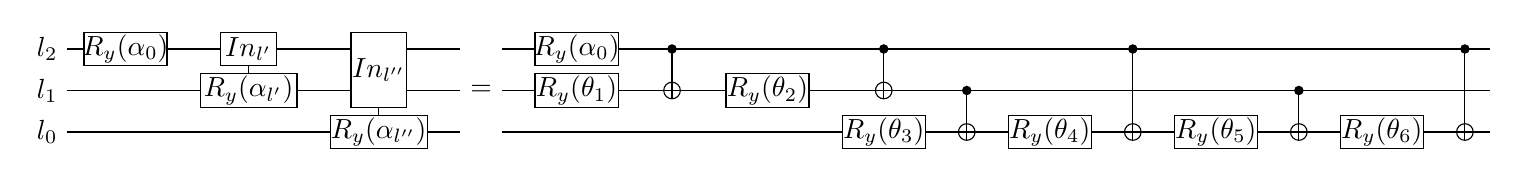
\begin{tikzpicture}[scale=1.000000,x=1pt,y=1pt]
\filldraw[color=white] (0.000000, -7.500000) rectangle (514.000000, 37.500000);
% Drawing wires
% Line 1: l2 W l_2
\draw[color=black] (0.000000,30.000000) -- (514.000000,30.000000);
\draw[color=black] (0.000000,30.000000) node[left] {$l_2$};
% Line 2: l1 W l_1
\draw[color=black] (0.000000,15.000000) -- (514.000000,15.000000);
\draw[color=black] (0.000000,15.000000) node[left] {$l_1$};
% Line 3: l0 W l_0
\draw[color=black] (0.000000,0.000000) -- (514.000000,0.000000);
\draw[color=black] (0.000000,0.000000) node[left] {$l_0$};
% Done with wires; drawing gates
% Line 5: l2 G:width=30 $R_y (\alpha_0)$
\begin{scope}
\draw[fill=white] (21.000000, 30.000000) +(-45.000000:21.213203pt and 8.485281pt) -- +(45.000000:21.213203pt and 8.485281pt) -- +(135.000000:21.213203pt and 8.485281pt) -- +(225.000000:21.213203pt and 8.485281pt) -- cycle;
\clip (21.000000, 30.000000) +(-45.000000:21.213203pt and 8.485281pt) -- +(45.000000:21.213203pt and 8.485281pt) -- +(135.000000:21.213203pt and 8.485281pt) -- +(225.000000:21.213203pt and 8.485281pt) -- cycle;
\draw (21.000000, 30.000000) node {$R_y (\alpha_0)$};
\end{scope}
% Line 6: l1 G:width=35 $R_y (\alpha_{l^\prime})$ l2 G:width=20 $In_{l^\prime}$
\draw (65.500000,30.000000) -- (65.500000,15.000000);
\begin{scope}
\draw[fill=white] (65.500000, 15.000000) +(-45.000000:24.748737pt and 8.485281pt) -- +(45.000000:24.748737pt and 8.485281pt) -- +(135.000000:24.748737pt and 8.485281pt) -- +(225.000000:24.748737pt and 8.485281pt) -- cycle;
\clip (65.500000, 15.000000) +(-45.000000:24.748737pt and 8.485281pt) -- +(45.000000:24.748737pt and 8.485281pt) -- +(135.000000:24.748737pt and 8.485281pt) -- +(225.000000:24.748737pt and 8.485281pt) -- cycle;
\draw (65.500000, 15.000000) node {$R_y (\alpha_{l^\prime})$};
\end{scope}
\begin{scope}
\draw[fill=white] (65.500000, 30.000000) +(-45.000000:14.142136pt and 8.485281pt) -- +(45.000000:14.142136pt and 8.485281pt) -- +(135.000000:14.142136pt and 8.485281pt) -- +(225.000000:14.142136pt and 8.485281pt) -- cycle;
\clip (65.500000, 30.000000) +(-45.000000:14.142136pt and 8.485281pt) -- +(45.000000:14.142136pt and 8.485281pt) -- +(135.000000:14.142136pt and 8.485281pt) -- +(225.000000:14.142136pt and 8.485281pt) -- cycle;
\draw (65.500000, 30.000000) node {$In_{l^\prime}$};
\end{scope}
% Line 7: l0 G:width=35 $R_y (\alpha_{l^{\prime\prime}})$ l2 l1 G:width=20 $In_{l^{\prime\prime}}$
\draw (112.500000,30.000000) -- (112.500000,0.000000);
\begin{scope}
\draw[fill=white] (112.500000, -0.000000) +(-45.000000:24.748737pt and 8.485281pt) -- +(45.000000:24.748737pt and 8.485281pt) -- +(135.000000:24.748737pt and 8.485281pt) -- +(225.000000:24.748737pt and 8.485281pt) -- cycle;
\clip (112.500000, -0.000000) +(-45.000000:24.748737pt and 8.485281pt) -- +(45.000000:24.748737pt and 8.485281pt) -- +(135.000000:24.748737pt and 8.485281pt) -- +(225.000000:24.748737pt and 8.485281pt) -- cycle;
\draw (112.500000, -0.000000) node {$R_y (\alpha_{l^{\prime\prime}})$};
\end{scope}
\begin{scope}
\draw[fill=white] (112.500000, 22.500000) +(-45.000000:14.142136pt and 19.091883pt) -- +(45.000000:14.142136pt and 19.091883pt) -- +(135.000000:14.142136pt and 19.091883pt) -- +(225.000000:14.142136pt and 19.091883pt) -- cycle;
\clip (112.500000, 22.500000) +(-45.000000:14.142136pt and 19.091883pt) -- +(45.000000:14.142136pt and 19.091883pt) -- +(135.000000:14.142136pt and 19.091883pt) -- +(225.000000:14.142136pt and 19.091883pt) -- cycle;
\draw (112.500000, 22.500000) node {$In_{l^{\prime\prime}}$};
\end{scope}
% Line 9: =
\draw[fill=white,color=white] (142.000000, -6.000000) rectangle (157.000000, 36.000000);
\draw (149.500000, 15.000000) node {$=$};
% Line 11: l2 G:width=30 $R_y (\alpha_0)$
\begin{scope}
\draw[fill=white] (184.000000, 30.000000) +(-45.000000:21.213203pt and 8.485281pt) -- +(45.000000:21.213203pt and 8.485281pt) -- +(135.000000:21.213203pt and 8.485281pt) -- +(225.000000:21.213203pt and 8.485281pt) -- cycle;
\clip (184.000000, 30.000000) +(-45.000000:21.213203pt and 8.485281pt) -- +(45.000000:21.213203pt and 8.485281pt) -- +(135.000000:21.213203pt and 8.485281pt) -- +(225.000000:21.213203pt and 8.485281pt) -- cycle;
\draw (184.000000, 30.000000) node {$R_y (\alpha_0)$};
\end{scope}
% Line 13: l1 G:width=30 $R_y (\theta_1)$
\begin{scope}
\draw[fill=white] (184.000000, 15.000000) +(-45.000000:21.213203pt and 8.485281pt) -- +(45.000000:21.213203pt and 8.485281pt) -- +(135.000000:21.213203pt and 8.485281pt) -- +(225.000000:21.213203pt and 8.485281pt) -- cycle;
\clip (184.000000, 15.000000) +(-45.000000:21.213203pt and 8.485281pt) -- +(45.000000:21.213203pt and 8.485281pt) -- +(135.000000:21.213203pt and 8.485281pt) -- +(225.000000:21.213203pt and 8.485281pt) -- cycle;
\draw (184.000000, 15.000000) node {$R_y (\theta_1)$};
\end{scope}
% Line 18: l0 LABEL
% Line 14: l2 +l1
\draw (218.500000,30.000000) -- (218.500000,15.000000);
\filldraw (218.500000, 30.000000) circle(1.500000pt);
\begin{scope}
\draw[fill=white] (218.500000, 15.000000) circle(3.000000pt);
\clip (218.500000, 15.000000) circle(3.000000pt);
\draw (215.500000, 15.000000) -- (221.500000, 15.000000);
\draw (218.500000, 12.000000) -- (218.500000, 18.000000);
\end{scope}
% Line 19: l0 LABEL
% Line 15: l1 G:width=30 $R_y (\theta_2)$
\begin{scope}
\draw[fill=white] (253.000000, 15.000000) +(-45.000000:21.213203pt and 8.485281pt) -- +(45.000000:21.213203pt and 8.485281pt) -- +(135.000000:21.213203pt and 8.485281pt) -- +(225.000000:21.213203pt and 8.485281pt) -- cycle;
\clip (253.000000, 15.000000) +(-45.000000:21.213203pt and 8.485281pt) -- +(45.000000:21.213203pt and 8.485281pt) -- +(135.000000:21.213203pt and 8.485281pt) -- +(225.000000:21.213203pt and 8.485281pt) -- cycle;
\draw (253.000000, 15.000000) node {$R_y (\theta_2)$};
\end{scope}
% Line 20: l0 LABEL
% Line 16: l2 +l1
\draw (295.000000,30.000000) -- (295.000000,15.000000);
\filldraw (295.000000, 30.000000) circle(1.500000pt);
\begin{scope}
\draw[fill=white] (295.000000, 15.000000) circle(3.000000pt);
\clip (295.000000, 15.000000) circle(3.000000pt);
\draw (292.000000, 15.000000) -- (298.000000, 15.000000);
\draw (295.000000, 12.000000) -- (295.000000, 18.000000);
\end{scope}
% Line 21: l0 G:width=30 $R_y (\theta_3)$
\begin{scope}
\draw[fill=white] (295.000000, -0.000000) +(-45.000000:21.213203pt and 8.485281pt) -- +(45.000000:21.213203pt and 8.485281pt) -- +(135.000000:21.213203pt and 8.485281pt) -- +(225.000000:21.213203pt and 8.485281pt) -- cycle;
\clip (295.000000, -0.000000) +(-45.000000:21.213203pt and 8.485281pt) -- +(45.000000:21.213203pt and 8.485281pt) -- +(135.000000:21.213203pt and 8.485281pt) -- +(225.000000:21.213203pt and 8.485281pt) -- cycle;
\draw (295.000000, -0.000000) node {$R_y (\theta_3)$};
\end{scope}
% Line 22: l1 +l0
\draw (325.000000,15.000000) -- (325.000000,0.000000);
\filldraw (325.000000, 15.000000) circle(1.500000pt);
\begin{scope}
\draw[fill=white] (325.000000, 0.000000) circle(3.000000pt);
\clip (325.000000, 0.000000) circle(3.000000pt);
\draw (322.000000, 0.000000) -- (328.000000, 0.000000);
\draw (325.000000, -3.000000) -- (325.000000, 3.000000);
\end{scope}
% Line 23: l0 G:width=30 $R_y (\theta_4)$
\begin{scope}
\draw[fill=white] (355.000000, -0.000000) +(-45.000000:21.213203pt and 8.485281pt) -- +(45.000000:21.213203pt and 8.485281pt) -- +(135.000000:21.213203pt and 8.485281pt) -- +(225.000000:21.213203pt and 8.485281pt) -- cycle;
\clip (355.000000, -0.000000) +(-45.000000:21.213203pt and 8.485281pt) -- +(45.000000:21.213203pt and 8.485281pt) -- +(135.000000:21.213203pt and 8.485281pt) -- +(225.000000:21.213203pt and 8.485281pt) -- cycle;
\draw (355.000000, -0.000000) node {$R_y (\theta_4)$};
\end{scope}
% Line 24: l2 +l0
\draw (385.000000,30.000000) -- (385.000000,0.000000);
\filldraw (385.000000, 30.000000) circle(1.500000pt);
\begin{scope}
\draw[fill=white] (385.000000, 0.000000) circle(3.000000pt);
\clip (385.000000, 0.000000) circle(3.000000pt);
\draw (382.000000, 0.000000) -- (388.000000, 0.000000);
\draw (385.000000, -3.000000) -- (385.000000, 3.000000);
\end{scope}
% Line 25: l0 G:width=30 $R_y (\theta_5)$
\begin{scope}
\draw[fill=white] (415.000000, -0.000000) +(-45.000000:21.213203pt and 8.485281pt) -- +(45.000000:21.213203pt and 8.485281pt) -- +(135.000000:21.213203pt and 8.485281pt) -- +(225.000000:21.213203pt and 8.485281pt) -- cycle;
\clip (415.000000, -0.000000) +(-45.000000:21.213203pt and 8.485281pt) -- +(45.000000:21.213203pt and 8.485281pt) -- +(135.000000:21.213203pt and 8.485281pt) -- +(225.000000:21.213203pt and 8.485281pt) -- cycle;
\draw (415.000000, -0.000000) node {$R_y (\theta_5)$};
\end{scope}
% Line 26: l1 +l0
\draw (445.000000,15.000000) -- (445.000000,0.000000);
\filldraw (445.000000, 15.000000) circle(1.500000pt);
\begin{scope}
\draw[fill=white] (445.000000, 0.000000) circle(3.000000pt);
\clip (445.000000, 0.000000) circle(3.000000pt);
\draw (442.000000, 0.000000) -- (448.000000, 0.000000);
\draw (445.000000, -3.000000) -- (445.000000, 3.000000);
\end{scope}
% Line 27: l0 G:width=30 $R_y (\theta_6)$
\begin{scope}
\draw[fill=white] (475.000000, -0.000000) +(-45.000000:21.213203pt and 8.485281pt) -- +(45.000000:21.213203pt and 8.485281pt) -- +(135.000000:21.213203pt and 8.485281pt) -- +(225.000000:21.213203pt and 8.485281pt) -- cycle;
\clip (475.000000, -0.000000) +(-45.000000:21.213203pt and 8.485281pt) -- +(45.000000:21.213203pt and 8.485281pt) -- +(135.000000:21.213203pt and 8.485281pt) -- +(225.000000:21.213203pt and 8.485281pt) -- cycle;
\draw (475.000000, -0.000000) node {$R_y (\theta_6)$};
\end{scope}
% Line 28: l2 +l0
\draw (505.000000,30.000000) -- (505.000000,0.000000);
\filldraw (505.000000, 30.000000) circle(1.500000pt);
\begin{scope}
\draw[fill=white] (505.000000, 0.000000) circle(3.000000pt);
\clip (505.000000, 0.000000) circle(3.000000pt);
\draw (502.000000, 0.000000) -- (508.000000, 0.000000);
\draw (505.000000, -3.000000) -- (505.000000, 3.000000);
\end{scope}
% Done with gates; drawing ending labels
% Done with ending labels; drawing cut lines and comments
% Done with comments
\end{tikzpicture}

    \caption{
        \textbf{Grover-Rudolph Circuit Compilation.} 
        An implementation of the Grover-Rudolph algorithm using several series of uniformly controlled rotations is shown when $L = 8$.
        This circuit requires $L - 1$ rotations when $L$ is a power of $2$ and the angles of the rotations are changed ($\theta_i \rightarrow \alpha_i$) based on classical preprocessing.
    }
    \label{fig:grover-rudolph}
\end{figure*}


The Grover-Rudolph algorithm can be thought of as performing several series of uniformly controlled rotations.
An example circuit diagram depicting this construction is shown in Figure \ref{fig:grover-rudolph}.
When $L$ is the number of probabilities (or coefficients) to prepare and is a power of $2$, this implementation uses $L-1$ uncontrolled rotations.
